{\bf [24 points] ChIP-seq analysis.}
\vspace{2mm}

We provide you some ChIP-seq peak data in \texttt{peak.bed} that contains the chromosome, start and end positions of the ChiP-seq peaks from an experiment. This is real transcription factor ChIP-Seq data from a cancer cell line, and your goal is to figure out if you can distinguish what transcription factor the experiment was performed with. In doing so, you will gain familiarity with some common genomics tools.
Most of the parts in this question are pretty open-ended; as long as your answers are well-supported, you will get credit.

\textbf{Data Processing Steps}

Using \texttt{peak.bed}, please complete the following tasks.
\begin{itemize}
\item Using your tool of choice, extract the first 100 lines of this file to a new file \texttt{"trimmed.bed"}.
\item 

        Load \texttt{"trimmed.bed"} in the UCSC Genome Browser (\url{https://genome.ucsc.edu}) as a custom track (use hg19 as the assembly). Get the genomic sequence for each of the intervals through UCSC Genome Browser. You can do that by going to Table Browser in UCSC Genome Browser, select custom track and load \texttt{"trimmed.bed"}, select output format as \textbf{sequence} and get output. Figure \ref{fig:genomebrowser} shows how to do this.

\begin{figure}[h]
\centering
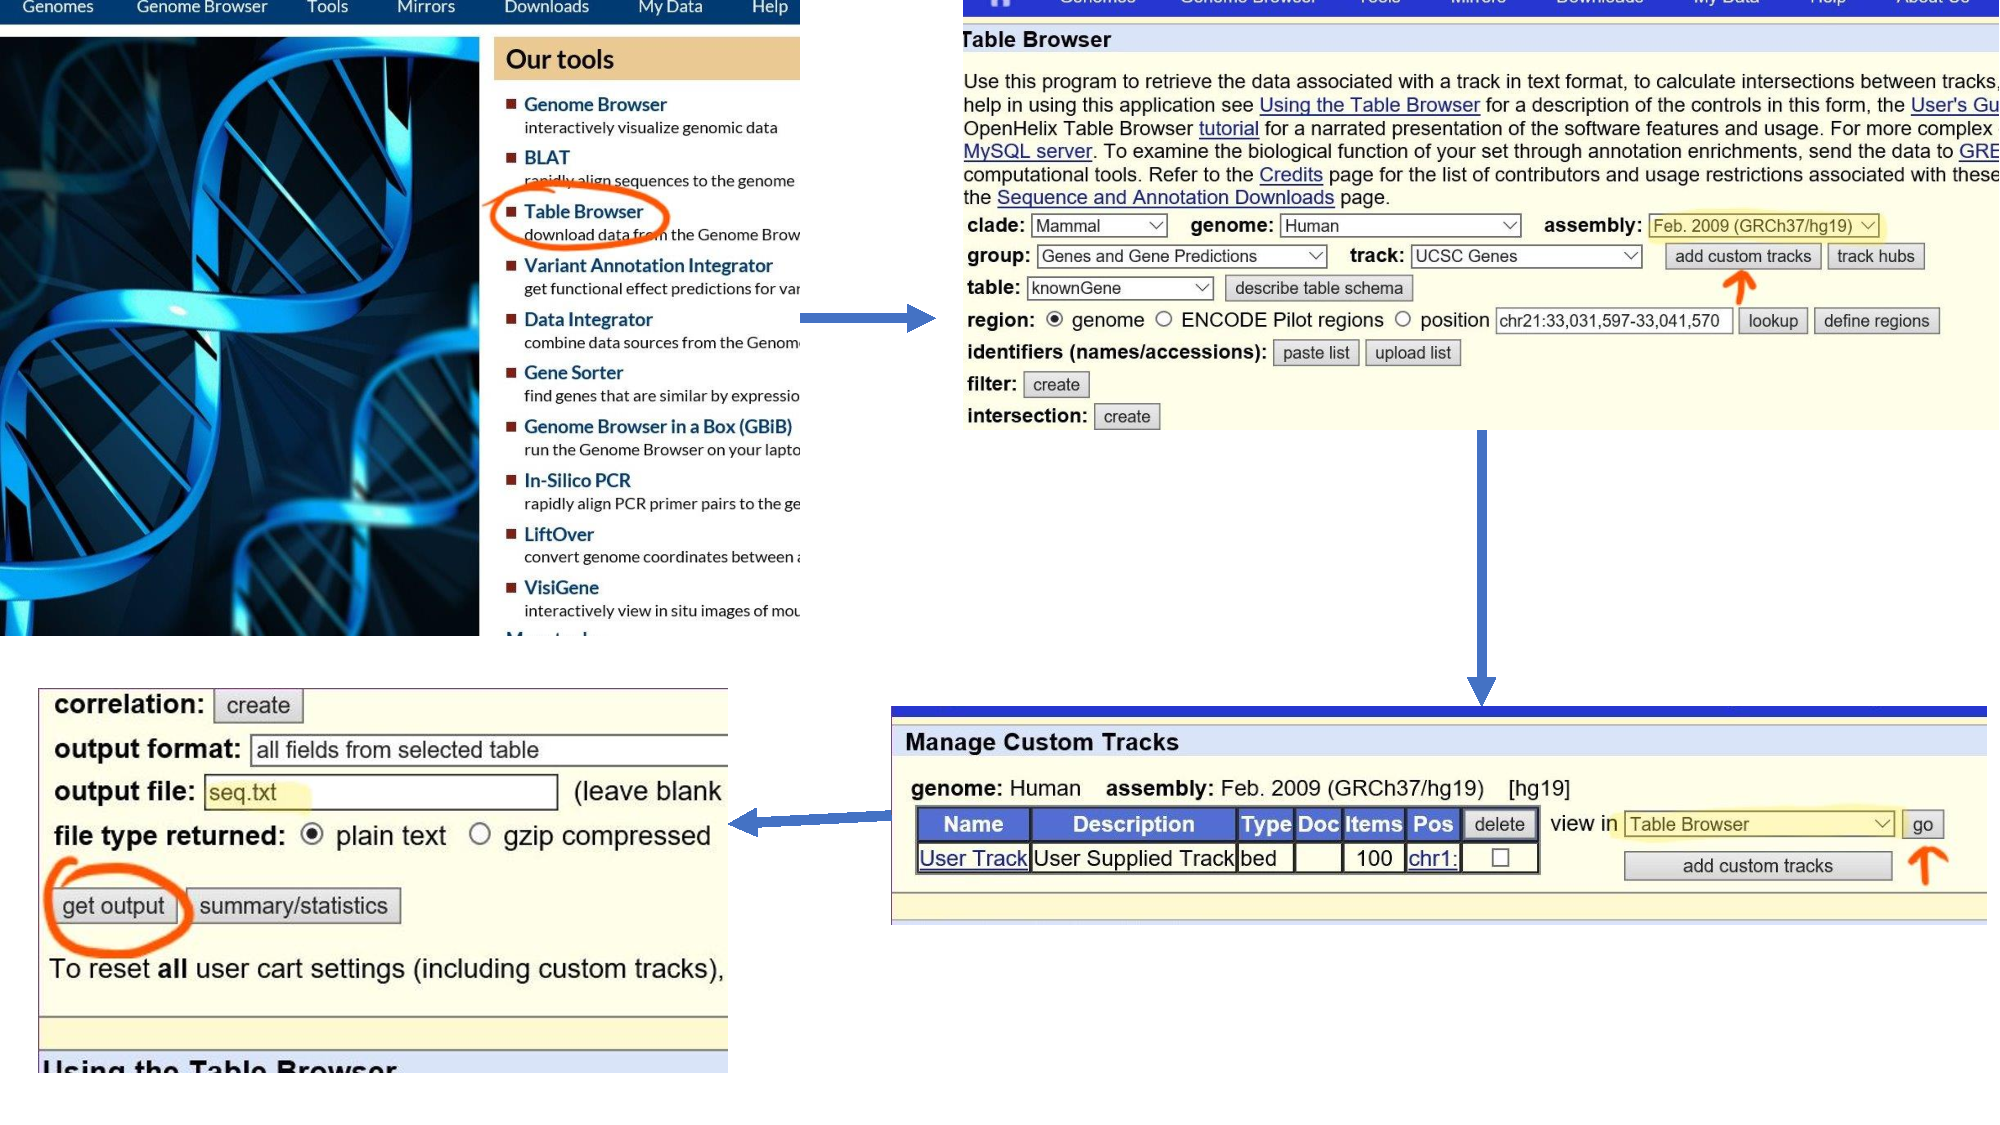
\includegraphics[width=0.8\textwidth]{tuts}
\caption{Use UCSC Table Browser to get the sequence.}
\label{fig:genomebrowser}
\end{figure}
    \item Use MEME (\url{http://meme-suite.org/tools/meme}) to call enriched motifs based on the output sequence. Use the default setting in MEME but only consider output motif with width from 5 to 9 (set under ``Advanced options''). Note that you may still need to adjust the size of the input file to keep the number of characters within 60,000 in the file. You may want to provide your email if you want a notification for when your results are ready from MEME. This may take some time, depending on the server load.
    \item Using each of your hits from MEME, feed them to TOMTOM by clicking the 'submit/download' arrow to the right of your MEME results. Use all default options for TOMTOM.
\end{itemize}



\textbf{Questions}
\begin{enumerate}

\item (2 points) Question -- Screenshot the output returned by MEME.  Based on the motif logos, which one is the most promising hit?


%%%%%%%%%%%%%%%%%%
\begin{solution}
\end{solution}
%%%%%%%%%%%%%%%%%%


\item (6 points) Question -- What is the top hit obtained from TomTom for each of the motifs from MEME? Based on this do you agree with your previous assessment? Note that the E-value reported by TOMTOM is the Bonferroni-corrected p-value.


%%%%%%%%%%%%%%%%%%
\begin{solution}
\end{solution}
%%%%%%%%%%%%%%%%%%


\item (8 points) Question -- Use the original peak.bed file and use GREAT (\url{http://great.stanford.edu/public/html/}) with default settings to identify enriched biological processes and pathways. \textbf{Be sure to use GREAT version 3.0.0, with species hg19.} Screenshot the top five Go Biological Process hits. How do these pathways compare to your expectations based on your MEME results? Would you consider these pathways statistically significant? Hint: explain what the important enrichment statistics mean.
 
 
%%%%%%%%%%%%%%%%%%
\begin{solution}
\end{solution}
%%%%%%%%%%%%%%%%%%


\item (2 points) Question -- Now take a quick look at the hits in the category MSigDB Preturbation category. Explain what type of data is shown here. How much might these hits depend on what type of cancer cells the experiment was done with?

%%%%%%%%%%%%%%%%%%
\begin{solution}
\end{solution}
%%%%%%%%%%%%%%%%%%

\item (6 points) Question -- Suppose that you were interested in determining what type of cancer the provided data was collected from.  Based on your GREAT analyses, how useful is the provided TF ChIP-Seq data for this purpose? Justify this with some explanation: this will require that you understand what the GO terms are, and what processes your TF(s) are involved with. Then outline a follow up high throughput sequencing experiment from those mentioned in class that might help you with this new objective. 

%%%%%%%%%%%%%%%%%%
\begin{solution}
\end{solution}
%%%%%%%%%%%%%%%%%%

\end{enumerate}
